\documentclass[11pt,a4paper]{article}
\usepackage[margin=23mm,headheight=14pt,headsep=8.5mm,footskip=10mm]{geometry}
\usepackage{amsmath,amssymb,amsthm}
\usepackage[no-math]{fontspec}
\usepackage{xeCJK}
\setmainfont{Latin Modern Roman}
\setCJKmainfont{FandolSong-Regular.otf}[Script=CustomDefault,Path=assets/fonts/fandol/,BoldFont=FandolSong-Bold.otf,ItalicFont=FandolSong-Regular.otf,BoldItalicFont=FandolSong-Bold.otf]
\setCJKsansfont{FandolSong-Regular.otf}[Script=CustomDefault,Path=assets/fonts/fandol/,BoldFont=FandolSong-Bold.otf]
\xeCJKsetup{PunctStyle=quanjiao,CheckSingle=true}
\usepackage{setspace}
\setstretch{1.12}
\setlength{\parindent}{2em}
\setlength{\parskip}{3pt}
\usepackage{titlesec}
\titleformat{\section}{\centering\normalfont\Large\bfseries}{\thesection.}{0.6em}{}
\titleformat{\subsection}{\normalfont\large\bfseries}{}{0pt}{}
\titlespacing*{\section}{0pt}{1.8\baselineskip}{1.0\baselineskip}
\titlespacing*{\subsection}{0pt}{1.1\baselineskip}{0.5\baselineskip}
\usepackage{enumitem}
\setlist[enumerate]{leftmargin=2em,labelsep=0.5em,itemsep=3pt,parsep=0pt,topsep=6pt}
\providecommand{\tightlist}{\setlength{\itemsep}{3pt}\setlength{\parskip}{0pt}}
\usepackage{needspace}
\newenvironment{statementblock}{\par\Needspace{9\baselineskip}\noindent}{\par\nopagebreak[4]}
\newenvironment{proofblock}{\par\Needspace{4\baselineskip}\noindent}{\par}
\usepackage{fancyhdr}
\pagestyle{fancy}
\fancyhf{}
\fancyhead[L]{\small 数学手记}
\fancyhead[R]{\small 复变函数 · 第一章}
\fancyfoot[C]{\thepage}
\renewcommand{\headrulewidth}{0.4pt}
\usepackage[hidelinks,unicode,bookmarksnumbered=true,linktoc=all]{hyperref}
\usepackage{bookmark}
\bookmarksetup{depth=2}
\hypersetup{pdftitle={复变函数讲义：第一章},pdfauthor={Vincent Arqain},pdfsubject={复数与复变函数}}
\renewcommand{\contentsname}{目录}
\setcounter{tocdepth}{1}
\setcounter{secnumdepth}{1}
\widowpenalty=10000
\clubpenalty=10000
\displaywidowpenalty=10000
\predisplaypenalty=10000
\interdisplaylinepenalty=10000
\raggedbottom

\usepackage{tabularx,booktabs,array}
\renewcommand{\thesection}{1.\arabic{section}}
\emergencystretch=2em

\usepackage{graphicx}
\usepackage{float}
\floatplacement{figure}{H}
\renewcommand{\figurename}{图}
\makeatletter
\def\maxwidth{\ifdim\Gin@nat@width>\linewidth\linewidth\else\Gin@nat@width\fi}
\def\maxheight{\ifdim\Gin@nat@height>0.72\textheight0.72\textheight\else\Gin@nat@height\fi}
\makeatother
\setkeys{Gin}{width=\maxwidth,height=\maxheight,keepaspectratio}
\providecommand{\pandocbounded}[1]{#1}
\setcounter{tocdepth}{2}
\begin{document}
\begin{center}
{\LARGE\bfseries 复变函数讲义\par}
\vspace{8pt}{\large 第一章\quad 复数与复变函数\par}
\vspace{6pt}{\small 依史济怀、刘太顺《复变函数》\quad 教材第 1—26 页\par}
\end{center}
\vspace{8pt}
本章含七节讲义及全部 63 道习题原题。定义、定理和性质沿用教材的记号与编号；
证明补足必要条件、退化情形与关键推导。教材未证的 Jordan 曲线定理给出拓扑证明，
并明确列出其同调论前置工具。习题不附解答，原题中的疑义另列校勘。
\tableofcontents
\clearpage
\section{复数的定义及其运算}
对应教材 §1.1，第 1---4 页。记号沿用教材：\(\mathbb C\)
为复数域，\(\bar z\) 为共轭，\(|z|\)
为模。先建立代数运算，再用模把它与极限连接。

\Needspace{5\baselineskip}
\subsection{复数域的构造}\label{ux590dux6570ux57dfux7684ux6784ux9020}

定义 \(\mathbb C=\{(a,b):a,b\in\mathbb R\}\)，并规定

\[
(a,b)+(c,d)=(a+c,b+d),\qquad
(a,b)(c,d)=(ac-bd,ad+bc).
\]

\textbf{性质：上述运算使 \(\mathbb C\) 成为域。}

证明：加法交换、结合及零元素 \((0,0)\)、负元素 \((-a,-b)\)
均逐坐标由实数运算得到。乘法交换由 \(ac-bd=ca-db\)、\(ad+bc=cb+da\)
得到。对第三个元素 \((e,f)\)，乘法两种结合次序的结果都是

\[
(ace-bde-adf-bcf,\;acf-bdf+ade+bce),
\]

故乘法结合。把乘法公式中 \(c,d\)
分别换成两项之和并展开，就得到分配律。单位元为 \((1,0)\)，且非零的
\((a,b)\) 满足

\[
(a,b)^{-1}=\left(\frac a{a^2+b^2},-\frac b{a^2+b^2}\right),
\]

代入乘法公式即得 \((1,0)\)，分母因 \((a,b)\ne(0,0)\)
而为正。全部域公理得证。

映射 \(a\mapsto(a,0)\)
保持加法、乘法与单位元且为单射，故把实数视为复数的子域。令
\(i=(0,1)\)，则 \(i^2=-1\)，且
\((a,b)=(a,0)+(b,0)i=a+bi\)；坐标唯一性给出这种表示的唯一性。

\textbf{定理 1.1.2：复数域不是有序域。}
这里``有序''要求全序与加法、正数乘法相容，不能只按实部、虚部的字典顺序排列。

证明：在任一有序域中，非零元 \(x\) 或 \(-x\) 为正，两者平方相同，故
\(x^2>0\)。于是 \(1=1^2>0\)，同时 \(-1=i^2>0\)；后式两边加 \(1\) 得
\(0>1\)，矛盾。

\Needspace{5\baselineskip}
\subsection{共轭与模}\label{ux5171ux8f6dux4e0eux6a21}

设 \(z=a+bi\)。定义
\(\operatorname{Re}z=a\)、\(\operatorname{Im}z=b\)、\(\bar z=a-bi\)、\(|z|=\sqrt{a^2+b^2}\)。

\textbf{命题 1.1.3：}

\[
\begin{aligned}
\operatorname{Re}z&=\frac{z+\bar z}{2},&
\operatorname{Im}z&=\frac{z-\bar z}{2i},\\
z\bar z&=|z|^2,&\overline{z+w}&=\bar z+\bar w,\\
\overline{zw}&=\bar z\bar w,&|zw|&=|z||w|,\\
|z/w|&=|z|/|w|\quad(w\ne0),&|\bar z|&=|z|.
\end{aligned}
\]

证明：头两式由 \(z+\bar z=2a\)、\(z-\bar z=2bi\) 得到。乘开得
\(z\bar z=a^2+b^2\)。令 \(w=c+di\)，加法的共轭等式两边都等于
\((a+c)-(b+d)i\)；乘法的共轭等式两边都等于 \((ac-bd)-(ad+bc)i\)。因而

\[
|zw|^2=zw\overline{zw}=z\bar z\,w\bar w=|z|^2|w|^2;
\]

两边取非负平方根得乘积公式，再对 \((z/w)w=z\)
应用该公式得商的公式。最后，\(|\bar z|^2=a^2+(-b)^2=|z|^2\)。这也给出常用的除法计算

\[
\frac{a+bi}{c+di}=\frac{ac+bd}{c^2+d^2}
+i\frac{bc-ad}{c^2+d^2},\qquad c+di\ne0.
\]

\Needspace{5\baselineskip}
\subsection{三角不等式及取等条件}\label{ux4e09ux89d2ux4e0dux7b49ux5f0fux53caux53d6ux7b49ux6761ux4ef6}

\textbf{命题 1.1.4：}
\(|\operatorname{Re}z|\le|z|\)、\(|\operatorname{Im}z|\le|z|\)，并且

\[
|z+w|\le|z|+|w|,\qquad
\bigl||z|-|w|\bigr|\le|z-w|.
\]

证明：前两式把 \(a^2,b^2\) 分别与 \(a^2+b^2\) 比较后开方即可。又

\[
\begin{aligned}
|z+w|^2&=|z|^2+2\operatorname{Re}(z\bar w)+|w|^2\\
&\le |z|^2+2|z||w|+|w|^2=(|z|+|w|)^2,
\end{aligned}
\]

故三角不等式成立。将 \(z=(z-w)+w\) 代入，得到 \(|z|-|w|\le|z-w|\)；交换
\(z,w\) 后合并即得反三角不等式。

取等当且仅当 \(z\bar w\) 是非负实数。若 \(w\ne0\)，这等价于
\(z/w\ge0\)；若
\(w=0\)，恒取等。因此准确的条件是：至少一数为零，或两数非零且同向。教材原句``存在
\(t\ge0\) 使 \(z=tw\)''必须另补 \(w=0\) 的情形。

\textbf{有限和形式：} 对 \(z_1,\ldots,z_n\in\mathbb C\)，

\[
\left|\sum_{j=1}^n z_j\right|\le\sum_{j=1}^n|z_j|.
\]

证明：从二项不等式反复应用即得。为判定等号，若总和 \(S\ne0\)，取
\(\eta=\bar S/|S|\)，则

\[
|S|=\sum_j\operatorname{Re}(\eta z_j)\le\sum_j|z_j|.
\]

每项差均非负，等号恰在所有 \(\eta z_j\)
都为非负实数时成立，即所有非零项方向相同。若 \(S=0\)，取等要求所有
\(z_j=0\)，也包含在上述条件中。

本节应掌握的构造是``乘以共轭''：它把乘除法、长度和取等条件化成实数运算；估计则先用三角不等式，精确判等时回到
\(\operatorname{Re}(z\bar w)\)。

\section{复数的几何表示}
对应教材 §1.2，第 4---11 页。非零复数写为
\(z=r(\cos\theta+i\sin\theta)\)，其中
\(r=|z|>0\)。\(\operatorname{Arg}z\) 是全部辐角组成的集合，\(\arg z\)
是唯一落在 \((-\pi,\pi]\) 中的主值。

\Needspace{5\baselineskip}
\subsection{乘除法就是旋转和伸缩}\label{ux4e58ux9664ux6cd5ux5c31ux662fux65cbux8f6cux548cux4f38ux7f29}

\textbf{性质：} 非零 \(z_1,z_2\)
的模相乘、辐角相加；相除时模相除、辐角相减。

证明：设
\(z_j=r_j(\cos\theta_j+i\sin\theta_j)\)。将乘积展开，利用三角和角公式得

\[
z_1z_2=r_1r_2\bigl(\cos(\theta_1+\theta_2)+i\sin(\theta_1+\theta_2)\bigr).
\]

取模便得乘积的模。辐角所有可能值均为 \(\theta_1+\theta_2+2k\pi\)，所以
\(\operatorname{Arg}(z_1z_2)=\operatorname{Arg}z_1+\operatorname{Arg}z_2\)
是集合等式。\(z_2^{-1}=r_2^{-1}(\cos(-\theta_2)+i\sin(-\theta_2))\)，代入乘法即得商的结论。主值一般只满足模
\(2\pi\) 相等，不能把集合等式直接改成主值等式。

复数的加减逐坐标进行，所以 \(z_2-z_1\) 表示由 \(z_1\) 指向 \(z_2\)
的位移，\(|z_2-z_1|\) 就是距离。乘以 \(w\ne0\) 把位移旋转 \(\arg w\)
并伸缩 \(|w|\) 倍。

\textbf{性质：} 非零位移 \(z_1,z_2\) 垂直当且仅当
\(\operatorname{Re}(z_1\bar z_2)=0\)；平行当且仅当
\(\operatorname{Im}(z_1\bar z_2)=0\)。

证明：写 \(z_j=x_j+iy_j\)，则实部为 \(x_1x_2+y_1y_2\)，即内积；虚部为
\(y_1x_2-x_1y_2\)，即二维行列式的相反数。内积为零刻画垂直，行列式为零刻画线性相关，从而刻画平行。

\Needspace{5\baselineskip}
\subsection{de Moivre
公式与开方}\label{de-moivre-ux516cux5f0fux4e0eux5f00ux65b9}

\textbf{性质：} 对任意整数 \(n\)，

\[
(\cos\theta+i\sin\theta)^n=\cos(n\theta)+i\sin(n\theta).
\]

证明：\(n=0\) 时两边均为 \(1\)；\(n\ge1\)
由刚证的乘法公式归纳得到。负指数由取倒数得到，而单位模复数的倒数就是共轭。

若 \(w=r(\cos\theta+i\sin\theta)\ne0\)，\(n\ge1\)，则方程 \(z^n=w\)
的全部根为

\[
z_k=r^{1/n}\left(\cos\frac{\theta+2k\pi}{n}
+i\sin\frac{\theta+2k\pi}{n}\right),\quad 0\le k<n.
\]

证明：令 \(z=\rho(\cos\varphi+i\sin\varphi)\)，原方程等价于
\(\rho^n=r\)、\(n\varphi=\theta+2k\pi\)。这些条件给出上式；两个所列根相等就要求指标之差为
\(n\) 的倍数，因而它们互不相同，也已穷尽所有根。\(w=0\) 时只有根
\(0\)，不能说有 \(n\) 个互异根。

令 \(\omega=\cos(2\pi/n)+i\sin(2\pi/n)\)，单位根为
\(1,\omega,\ldots,\omega^{n-1}\)，任一非零复数的 \(n\)
次根都是某一根乘以这些单位根。对 \(n\ge2\)，

\[
1+\omega+\cdots+\omega^{n-1}=\frac{1-\omega^n}{1-\omega}=0,
\]

故正 \(n\) 边形顶点的复数和为零；这里明确用了 \(\omega\ne1\)。

\Needspace{5\baselineskip}
\subsection{两个几何判据}\label{ux4e24ux4e2aux51e0ux4f55ux5224ux636e}

\textbf{圆与直线的统一方程：} 设
\(a,d\in\mathbb R\)、\(\beta\in\mathbb C\)，考察

\[
a|z|^2+\bar\beta z+\beta\bar z+d=0.
\]

证明：当 \(a=0,\beta\ne0\)，它是
\(2\operatorname{Re}(\bar\beta z)+d=0\)，即直线。当 \(a\ne0\)，配方得到

\[
\left|z+\frac\beta a\right|^2=\frac{|\beta|^2-ad}{a^2}.
\]

右边为正时是圆周，等于零时是一个点，小于零时无解。因此称``圆''时必须保留正半径条件。

\textbf{例 1.2.2 的准确形式：} 四个互异点 \(z_1,z_2,z_3,z_4\)
共圆或共线，当且仅当

\[
\frac{z_1-z_3}{z_1-z_4}\bigg/\frac{z_2-z_3}{z_2-z_4}\in\mathbb R.
\]

证明：固定 \(z_2,z_3,z_4\)，记 \(c=(z_2-z_3)/(z_2-z_4)\ne0\)。条件等价于

\[
\operatorname{Im}\bigl(\bar c(z-z_3)(\bar z-\bar z_4)\bigr)=0.
\]

展开后是上述圆或直线型的实方程。它不是恒等式：映射 \((z-z_3)/(z-z_4)\)
的逆式为 \(z=(tz_4-z_3)/(t-1)\)，取 \(t\) 不在实直线 \(c\mathbb R\)
上即可找到不满足条件的 \(z\)。该轨迹含
\(z_2,z_3,z_4\)，故既非空集也非独点集，只能是通过三点的圆或直线。非共线三点唯一确定圆，共线三点唯一确定直线；再代入
\(z=z_1\)
即得双向结论。教材将``共圆''作为结论时应补充``不共线''，否则四个互异实数便是反例。

\Needspace{5\baselineskip}
\subsection{中点构造的计算}\label{ux4e2dux70b9ux6784ux9020ux7684ux8ba1ux7b97}

教材例 1.2.1 中，\(AB=AC\)，\(P,Q\) 位于 \(AB\)，\(R,S\) 位于 \(AC\)，且
\(PQ=RS=h\)；\(M,N\) 分别为 \(PR,QS\) 中点。取
\(A=0\)，\(B=b>0\)，\(C=b(\cos\theta+i\sin\theta)\)。记
\(\eta=\cos\theta+i\sin\theta\)，则
\(P=a,Q=a+h,R=r\eta,S=(r+h)\eta\)，从而

\[
N-M=\frac h2(1+\eta),\qquad C-B=b(\eta-1).
\]

证明：中点坐标由两端点相加除以 \(2\) 得到，所以第一式中 \(a,r\)
均消去。又 \(|\eta|=1\)，故

\[
(N-M)\overline{(C-B)}
=\frac{bh}{2}(1+\eta)(\bar\eta-1)
=\frac{bh}{2}(\bar\eta-\eta)
\]

是纯虚数，按垂直判据即得 \(MN\perp BC\)。教材第 7 页中间一式多出的 \(r\)
不应保留。

几何题的切入点是选原点和实轴，让旋转写成同一个单位复数、让中点写成平均值；之后先消去位置参数，再判实部或虚部。

\section{扩充平面与复数的球面表示}
对应教材 §1.3，第 11---13 页。扩充复平面记为
\(\mathbb C_\infty=\mathbb C\cup\{\infty\}\)，只有一个无穷远点；它不是有序实数轴上的正、负无穷。

\Needspace{5\baselineskip}
\subsection{扩充平面不是一个更大的域}\label{ux6269ux5145ux5e73ux9762ux4e0dux662fux4e00ux4e2aux66f4ux5927ux7684ux57df}

对有限 \(z\) 约定 \(z\pm\infty=\infty\)、\(z/\infty=0\)；对有限非零
\(z\) 约定
\(z\cdot\infty=\infty\)、\(z/0=\infty\)。\(0\cdot\infty\)、\(0/0\)、\(\infty/\infty\)、\(\infty-\infty\)
都没有定义。这些是延拓记号，不服从域中的全部消去规则。例如若允许对
\(1+\infty=\infty\) 消去 \(\infty\)，就会得到 \(1=0\)。

\Needspace{5\baselineskip}
\subsection{球极投影公式}\label{ux7403ux6781ux6295ux5f71ux516cux5f0f}

取单位球面 \(S\subset\mathbb R^3\)，北极 \(N=(0,0,1)\)，复平面对应
\(x_3=0\)。从北极投影得到 \(z=x+iy\) 的球面像 \(P(z)\)。

\textbf{性质：}

\[
P(z)=\left(\frac{2x}{1+|z|^2},\frac{2y}{1+|z|^2},
\frac{|z|^2-1}{1+|z|^2}\right),\qquad P(\infty)=N.
\]

证明：直线 \(N+t((x,y,0)-N)\) 的坐标是 \((tx,ty,1-t)\)。代入球面方程得

\[
t^2(|z|^2+1)-2t=0.
\]

根 \(t=0\) 对应北极，另一根为 \(2/(1+|z|^2)\)，代回即得。若
\(P=(x_1,x_2,x_3)\ne N\)，逆公式为

\[
z=\frac{x_1+ix_2}{1-x_3}.
\]

因为 \(x_1^2+x_2^2=(1-x_3)(1+x_3)\)，代入可恢复
\(P\)。因此该对应为双射。公式也直接说明：\(|z|<1\)、\(=1\)、\(>1\)
分别对应南半球、赤道、北半球。

\Needspace{5\baselineskip}
\subsection{弦距与无穷远点的邻域}\label{ux5f26ux8dddux4e0eux65e0ux7a77ux8fdcux70b9ux7684ux90bbux57df}

\textbf{性质：} 球面像间的欧氏距离为

\[
\begin{aligned}
q(z,w)&=\frac{2|z-w|}{\sqrt{(1+|z|^2)(1+|w|^2)}},\\
q(z,\infty)&=\frac2{\sqrt{1+|z|^2}}.
\end{aligned}
\]

证明：\(|P(z)|=|P(w)|=1\)，故距离平方为
\(2-2P(z)\cdot P(w)\)。将点积写出，分子化简为
\(4(|z|^2+|w|^2-2\operatorname{Re}(z\bar w))=4|z-w|^2\)，得到第一式。第二式直接计算
\(|P(z)-N|\)
即得。由于这是三维距离经双射拉回，正定性、对称性及三角不等式均成立。

由第二式，\(z_n\to\infty\) 等价于 \(|z_n|\to+\infty\)，也等价于
\(q(z_n,\infty)\to0\)；对非零的有限项，又等价于 \(1/z_n\to0\)。对有限
\(z_0\)，欧氏收敛蕴含弦距收敛。反过来，弦距收敛先使 \(P(z_n)\)
留在远离北极的邻域，再由逆公式的连续性得到欧氏收敛。

教材记 \(B(\infty;R)=\{z\in\mathbb C:|z|>R\}\)。在 \(\mathbb C_\infty\)
中真正包含中心的邻域应写成
\(B(\infty;R)\cup\{\infty\}\)。这样无穷远点与有限点在拓扑上没有特殊待遇。

\Needspace{5\baselineskip}
\subsection{圆与直线为何统一}\label{ux5706ux4e0eux76f4ux7ebfux4e3aux4f55ux7edfux4e00}

\textbf{性质：}
球面上的非退化圆周在投影下对应复平面的圆周，或加上无穷远点的直线，反之亦然。

证明：球面圆周是球面与平面 \(Ax_1+Bx_2+Cx_3=D\)
的非退化交线。代入投影公式并乘以 \(1+|z|^2\)，得到

\[
(C-D)|z|^2+2Ax+2By-(C+D)=0.
\]

若 \(C\ne D\)，它是圆型方程；原交线非退化，故确为正半径圆周。若
\(C=D\)，平面过北极，\(A,B\)
不同时为零，得到直线；北极恰补上其无穷远点。反过来，任一圆或直线方程都能按此形式选择
\(A,B,C,D\)，于是得到相应球面圆周。

球面表示的作用是统一``有限处''和``无穷远处''的讨论；计算无穷远行为时，优先换坐标
\(\zeta=1/z\)。

\section{复数列的极限}
对应教材 §1.4，第 13---15 页。有限极限的定义是：任给
\(\varepsilon>0\)，存在 \(N\)，当 \(n>N\) 时
\(|z_n-z_0|<\varepsilon\)。趋于 \(\infty\)
则要求模最终大于任意给定的正数。

\Needspace{5\baselineskip}
\subsection{收敛等价于两个实坐标分别收敛}\label{ux6536ux655bux7b49ux4ef7ux4e8eux4e24ux4e2aux5b9eux5750ux6807ux5206ux522bux6536ux655b}

\textbf{性质：} 若 \(z_n=x_n+iy_n\)、\(z_0=x_0+iy_0\)，则 \(z_n\to z_0\)
当且仅当 \(x_n\to x_0\) 且 \(y_n\to y_0\)。

证明：一方面 \(|x_n-x_0|,|y_n-y_0|\le|z_n-z_0|\)；另一方面
\(|z_n-z_0|\le|x_n-x_0|+|y_n-y_0|\)。必要性由前两式得到，充分性对两坐标分别用误差
\(\varepsilon/2\) 即得。

\textbf{性质：} 有限极限唯一，收敛列有界，任一子列收敛于同一极限。

证明：若同时收敛于 \(a,b\)，则 \(|a-b|\le|a-z_n|+|z_n-b|\to0\)，故
\(a=b\)。取误差 \(1\)，尾项满足
\(|z_n|\le|a|+1\)，再把有限个首项的模纳入上界，得到有界性。给定误差后，子列的指标最终超过原列所需的
\(N\)，故子列仍趋于 \(a\)。

\Needspace{5\baselineskip}
\subsection{极限与代数运算}\label{ux6781ux9650ux4e0eux4ee3ux6570ux8fd0ux7b97}

\textbf{性质：} 若 \(z_n\to z\)、\(w_n\to w\)
均为有限极限，则和、差、积分别趋于 \(z+w,z-w,zw\)；若
\(w\ne0\)，商最终有定义并趋于 \(z/w\)。此外
\(\bar z_n\to\bar z\)、\(|z_n|\to|z|\)。

证明：和与差由三角不等式得到。因 \(z_n\) 有界，

\[
|z_nw_n-zw|\le |z_n|\,|w_n-w|+|w|\,|z_n-z|\longrightarrow0.
\]

若 \(w\ne0\)，最终 \(|w_n|\ge|w|/2\)，从而

\[
\left|\frac1{w_n}-\frac1w\right|
=\frac{|w_n-w|}{|w_n||w|}
\le\frac{2|w_n-w|}{|w|^2}\longrightarrow0;
\]

再与积的结论结合。共轭的误差满足
\(|\bar z_n-\bar z|=|z_n-z|\)；模的误差由反三角不等式控制。

\Needspace{5\baselineskip}
\subsection{Cauchy
准则与完备性}\label{cauchy-ux51c6ux5219ux4e0eux5b8cux5907ux6027}

称 \(\{z_n\}\) 为 Cauchy 列，是指任给 \(\varepsilon>0\)，存在
\(N\)，对所有 \(m,n>N\) 都有 \(|z_n-z_m|<\varepsilon\)。

\textbf{定理：} 复数列收敛于有限复数，当且仅当它是 Cauchy 列。因此
\(\mathbb C\) 在欧氏距离下完备。

证明：若 \(z_n\to z\)，分别使
\(|z_n-z|,|z_m-z|<\varepsilon/2\)，由三角不等式得到 Cauchy
条件。反之，由

\[
|x_n-x_m|\le|z_n-z_m|,\qquad
|y_n-y_m|\le|z_n-z_m|
\]

知实部列、虚部列均为实 Cauchy 列。由实数完备性，分别存在实极限
\(x,y\)；逐坐标收敛判据遂给出 \(z_n\to x+iy\)。

趋于无穷远的列在欧氏距离下不是 Cauchy 列，因为 Cauchy
列有界：令尾项彼此距离小于 \(1\)，固定其中一项即可控制整个尾列。

\Needspace{5\baselineskip}
\subsection{辐角不能在割线上随意取极限}\label{ux8f90ux89d2ux4e0dux80fdux5728ux5272ux7ebfux4e0aux968fux610fux53d6ux6781ux9650}

模连续，但主辐角在负实轴处存在跳跃。例如
\(z_n=-1+i(-1)^n/n\to-1\)，两侧主辐角分别趋近 \(\pi\) 与
\(-\pi\)，故主辐角列不收敛。

\textbf{性质：} 若 \(z_0\notin(-\infty,0]\) 且所有 \(z_n\ne0\)，则
\(z_n\to z_0\) 等价于 \(|z_n|\to|z_0|\) 和 \(\arg z_n\to\arg z_0\)。

证明：在割平面上，有显式公式

\[
\arg(x+iy)=2\arctan\frac{y}{\sqrt{x^2+y^2}+x}.
\]

分母为正，右边连续；由半角公式可核验其正弦、余弦正好为
\(y/|z|,x/|z|\)，且值在 \((-\pi,\pi)\)，故等于主辐角。若
\(z_n\to z_0\)，尾项处于这个开集，得到所需极限；反向将极限代入
\(z_n=|z_n|(\cos\arg z_n+i\sin\arg z_n)\) 即得。

判断复数列收敛，优先选择坐标、模与辐角或 Cauchy
条件中最便于估计的一种；使用辐角前先检查极限是否落在割线上。

\section{开集、闭集和紧集}
对应教材 §1.5，第 15---20 页。除特别注明，内部、闭包、边界、导集均相对于
\(\mathbb C\)；改在 \(\mathbb C_\infty\) 中讨论时，无穷远点必须计入。

\Needspace{5\baselineskip}
\subsection{从邻域定义读出集合运算}\label{ux4eceux90bbux57dfux5b9aux4e49ux8bfbux51faux96c6ux5408ux8fd0ux7b97}

\(B(a;r)=\{z:|z-a|<r\}\)，\(r>0\)。若某邻域包含于 \(E\)，\(a\)
是内点；若包含于
\(E^c\)，是外点；每一邻域都同时遇到两者时，是边界点。分别记内部
\(E^\circ\)、边界 \(\partial E\)。每个去心邻域都遇到 \(E\)
的点称为极限点，极限点全体为导集 \(E'\)；闭包为
\(\bar E=E\cup E'\)。属于 \(E\) 而非 \(E'\)
的点称孤立点。开集的每个点都是内点，闭集的补集是开集。

\textbf{命题 1.5.1 及直接性质：}

\[
\begin{aligned}
a\in\bar E&\iff B(a;r)\cap E\ne\varnothing\quad(\forall r>0),\\
(\bar E)^c&=(E^c)^\circ,\qquad
\overline{E^c}=(E^\circ)^c,\\
\mathbb C&=E^\circ\mathbin{\dot\cup}(E^c)^\circ\mathbin{\dot\cup}\partial E,\\
\partial E&=\bar E\cap\overline{E^c}=\bar E\setminus E^\circ.
\end{aligned}
\]

证明：若 \(a\in E\)，每个邻域因包含 \(a\) 而遇到 \(E\)；若
\(a\in E'\)，由极限点定义仍然如此。反之，若每个邻域都遇到 \(E\) 而
\(a\notin E\)，这些交点都不同于 \(a\)，故
\(a\in E'\)。对这个判据取否定，便得到第一个补集等式；再把 \(E\) 换成
\(E^c\)
并取补，得到第二式。内点、外点互斥，两者均不是时正好是边界点，由此得到不交分解及边界两式。

\textbf{命题 1.5.2：} \(E^\circ\) 开，\(\bar E,\partial E\) 闭；\(E\)
闭当且仅当 \(E=\bar E\)，也当且仅当 \(E'\subset E\)。

证明：若 \(B(a;r)\subset E\)，则其中任一点 \(b\) 的邻域 \(B(b;r-|b-a|)\)
仍包含于 \(E\)，故
\(B(a;r)\subset E^\circ\)。这证明内部开。由补集等式，\(\bar E\)
的补集开，故闭；边界的补集为两个开集的并，故也开。若 \(E\)
闭，\(E^c=(E^c)^\circ=(\bar E)^c\)，故
\(E=\bar E\)；反向直接用闭包的闭性。最后利用 \(\bar E=E\cup E'\)
得到导集判据。

\textbf{性质：} 任意并与有限交保持开性；任意交与有限并保持闭性。

证明：并集中一点属于某个开集，该开集提供所需邻域。有限交中一点在每个开集都有正邻域半径，取这些半径的最小值。闭集的结论由取补和
de Morgan 等式得到。无限交不一定开，例如
\(\bigcap_{n\ge1}B(0;1/n)=\{0\}\)。

\textbf{序列判据：} \(a\in\bar E\) 当且仅当有 \(E\) 中序列趋于
\(a\)；因此 \(E\) 闭当且仅当包含自身全部收敛序列的有限极限。

证明：在每个 \(B(a;1/n)\) 中选取 \(z_n\in E\)，则 \(z_n\to a\)。反之，若
\(z_n\to a\)，每个邻域含某个 \(z_n\)，故 \(a\in\bar E\)。结合
\(E=\bar E\) 即得闭集判据。该序列可以恒等于 \(a\)；若要刻画导集，应要求
\(z_n\ne a\)。

\Needspace{5\baselineskip}
\subsection{Cantor
闭集套定理}\label{cantor-ux95edux96c6ux5957ux5b9aux7406}

\textbf{定理 1.5.3：} 非空闭集满足 \(F_1\supset F_2\supset\cdots\) 且
\(\operatorname{diam}F_n\to0\)，则 \(\bigcap_nF_n\) 恰含一点。这里
\(\operatorname{diam}F=\sup_{z,w\in F}|z-w|\)。

证明：选 \(z_n\in F_n\)。对 \(m,n\ge N\)，两点都在 \(F_N\)，故
\(|z_n-z_m|\le\operatorname{diam}F_N\to0\)。由完备性
\(z_n\to z_0\)。固定 \(k\)，尾列全在闭集 \(F_k\)，故
\(z_0\in F_k\)，于是 \(z_0\) 属于交集。若 \(w\) 也属于交集，则
\(|z_0-w|\le\operatorname{diam}F_n\) 对所有 \(n\) 成立，故 \(w=z_0\)。

闭性保证极限留在集合内，直径趋零同时负责 Cauchy
性和唯一性，缺少两者中的任一个都不能套用结论。

\Needspace{5\baselineskip}
\subsection{Heine--Borel 定理}\label{heineborel-ux5b9aux7406}

紧集指任一开覆盖都有有限子覆盖的集合。空集和有限集显然紧：分别不选集合，或每个点选一个覆盖集。

\textbf{定理 1.5.5：} 在 \(\mathbb C\) 中，紧性等价于有界闭性；在
\(\mathbb C_\infty\) 中，紧性等价于闭性。

证明：设 \(E\subset\mathbb C\) 紧。开覆盖 \(\{B(0;n):n\ge1\}\)
有有限子覆盖，故 \(E\) 有界。对 \(a\notin E\)，以
\(B(z;|z-a|/3)\)（\(z\in E\)）覆盖 \(E\)，取有限子覆盖，设中心为
\(z_1,\ldots,z_m\)。这些圆盘到 \(a\) 的距离至少分别为
\(2|z_j-a|/3\)；取它们的正最小值，便得到不遇到 \(E\) 的 \(a\)
的邻域。因此 \(E^c\) 开，\(E\) 闭。

反之，设 \(E\) 有界闭而某开覆盖没有有限子覆盖。取闭正方形 \(Q\) 包含
\(E\)，四等分后至少有一块 \(Q_1\) 与 \(E\)
的交不能被有限覆盖，否则四块的有限覆盖合起来就覆盖
\(E\)。反复四等分，得到非空闭集
\(F_n=E\cap Q_n\)，彼此嵌套、直径趋零，且都不能有限覆盖。由 Cantor
定理，交集为 \(\{a\}\)。原开覆盖中某个 \(G\) 含 \(a\)，于是有
\(B(a;r)\subset G\)；当 \(n\)
大时，\(F_n\subset B(a;r)\subset G\)，一个集合便覆盖 \(F_n\)，矛盾。

在球面上，用弦距重复``紧集的补集开''的论证即知紧集闭。反之，设 \(E\)
在扩充平面闭。若不含 \(\infty\)，其补集含无穷远邻域，故 \(E\)
有界，归结到刚证的平面情形。若包含 \(\infty\)，从任意开覆盖选一个包含
\(\infty\) 的开集 \(G\)；\(E\setminus G\) 是不含 \(\infty\)
的球面闭集，因而是平面上的有界闭集，可由有限个原覆盖集覆盖，再加 \(G\)
即可。

\Needspace{5\baselineskip}
\subsection{紧性产生统一的正距离}\label{ux7d27ux6027ux4ea7ux751fux7edfux4e00ux7684ux6b63ux8dddux79bb}

对非空集合定义
\(d(E,F)=\inf\{|z-w|:z\in E,w\in F\}\)，\(d(a,F)=d(\{a\},F)\)。

\textbf{定理 1.5.6：} 非空紧集 \(E\) 与非空闭集 \(F\) 不相交，则
\(d(E,F)>0\)。

证明：每个 \(a\in E\) 都在 \(F^c\) 中，故 \(d(a,F)>0\)。圆盘
\(B(a;d(a,F)/2)\) 覆盖 \(E\)，取有限子覆盖，中心为
\(a_1,\ldots,a_m\)，令 \(\delta=\min_jd(a_j,F)/2>0\)。任意 \(z\in E\)
属于某个圆盘，故对 \(w\in F\)，

\[
|z-w|\ge |a_j-w|-|z-a_j|\ge\frac{d(a_j,F)}2\ge\delta.
\]

取下确界即得。若空集出现，可约定与空集距离为
\(+\infty\)，但存在取到距离的点的结论必须排除空集。

紧性不能只换成闭性：\(E=\mathbb R\) 与
\(F=\{x+i\mathrm e^x:x\in\mathbb R\}\) 不交，且距离为零。\(F\)
闭，因为其中点若有有限复极限，实部必趋于有限 \(x\)，虚部就趋于
\(\mathrm e^x\)；而 \(x\to-\infty\) 时高度趋零。

\Needspace{5\baselineskip}
\subsection{Bolzano--Weierstrass
定理}\label{bolzanoweierstrass-ux5b9aux7406}

\textbf{定理 1.5.7：}
无穷点集在扩充平面中至少有一个极限点；有界无穷点集在有限平面中有极限点。

证明：无界时可选 \(z_n\in E\) 满足 \(|z_n|>n\)，故 \(\infty\)
是极限点。有界时若没有有限极限点，则 \(E'=\varnothing\)，故 \(E\)
闭而紧。每个 \(z\in E\) 都有仅含它自身一个 \(E\)
中点的邻域。这些邻域的有限子覆盖只能覆盖有限个点，与 \(E\) 无穷矛盾。

\textbf{推论：}
有界复数列有收敛子列，紧集中的序列有极限仍在该集内的收敛子列。

证明：若某值出现无穷多次，取常值子列；否则值集无穷且有界，取其极限点
\(a\)。每个 \(B(a;1/k)\)
中都有无穷多个不同值，因此可逐次选取严格递增指标 \(n_k\) 使
\(|z_{n_k}-a|<1/k\)。若原列位于紧集，闭性保证 \(a\) 仍在其中。

全节的主线是：实数完备性给复数完备性，完备性给闭集套，闭集套给有限覆盖，有限覆盖再把逐点控制变成全体上的统一控制。

\section{曲线和域}
对应教材 §1.6，第 21---24 页。连续曲线是映射
\(\gamma:[a,b]\to\mathbb C\)，轨迹记
\(\gamma^*=\{\gamma(t):a\le t\le b\}\)。曲线保留参数次序；轨迹只是点集，二者不能混淆。

\Needspace{5\baselineskip}
\subsection{曲线、方向与长度}\label{ux66f2ux7ebfux65b9ux5411ux4e0eux957fux5ea6}

参数增大给出曲线方向，\(\gamma(a),\gamma(b)\)
为起点、终点；二者相同时是闭曲线。除首尾可能相同外没有重复点，是简单曲线或简单闭曲线。简单闭曲线又称围道。

\textbf{性质：} 连续曲线的轨迹紧。

证明：任取轨迹的开覆盖，原像给出闭区间 \([a,b]\)
的相对开覆盖；由实区间的紧性取有限子覆盖，再取对应的原覆盖集便覆盖轨迹。

对分割 \(a=t_0<\cdots<t_n=b\)，内接折线长为
\(\sum_j|\gamma(t_j)-\gamma(t_{j-1})|\)。这些长度有有限上界时称曲线可求长，长度为其上确界。加分点只会增大或保持折线长，因为每条旧弦由新弦之和估计。

若 \(\gamma(t)=x(t)+iy(t)\) 为 \(C^1\) 且
\(\gamma'(t)\ne0\)，称光滑曲线，切向量为 \(\gamma'(t)\)，其方向为
\(\operatorname{Arg}\gamma'(t)\)。这是因为差商
\([\gamma(t+h)-\gamma(t)]/h\to\gamma'(t)\)，按长度归一后，正向弦的方向趋于导数的方向。

\textbf{性质：} \(C^1\) 曲线可求长，且

\[
\ell(\gamma)=\int_a^b|\gamma'(t)|\,dt
=\int_a^b\sqrt{x'(t)^2+y'(t)^2}\,dt.
\]

证明：逐坐标用微积分基本定理，再用向量积分的三角不等式，得任一内接折线长不超过右端。后一不等式也可由
Riemann 和的三角不等式取极限得到。反向，设 \(\omega(\delta)\) 是连续函数
\(\gamma'\) 的模连续度，\(\omega(\delta)\to0\)。网格不超过 \(\delta\)
的分割上，任取 \(\tau_j\in[t_{j-1},t_j]\)，有

\[
\left|\gamma(t_j)-\gamma(t_{j-1})-\gamma'(\tau_j)(t_j-t_{j-1})\right|
\le\omega(\delta)(t_j-t_{j-1}).
\]

由反三角不等式求和，折线长至少为对应的 \(|\gamma'|\) 的 Riemann 和减去
\(\omega(\delta)(b-a)\)。令网格趋零，得到反向不等式。对逐段光滑曲线，在分段点处拆开，各段长度相加；因细分不减小折线长，长度定义也确实具有这种可加性。

\Needspace{5\baselineskip}
\subsection{连通的两个刻画}\label{ux8fdeux901aux7684ux4e24ux4e2aux523bux753b}

教材定义：非空点集 \(E\) 连通，是指每当 \(E=E_1\cup E_2\)
是两个不交非空集的分解，就有 \(E_1\cap\bar E_2\ne\varnothing\) 或
\(\bar E_1\cap E_2\ne\varnothing\)。等价地，不能分成两个不交非空的相对开集。

证明：若上述两交集都空，则每个 \(E_1\) 中点有避开 \(E_2\) 的邻域，故
\(E_1\) 相对开，\(E_2\)
同理；反之，相对开分解使每点都存在避开另一部分的相对邻域，故这两个交集都空。

\textbf{命题 1.6.2：} 开集 \(E\)
连通，当且仅当不能表示为两个不交非空开集的并。

证明：因 \(E\) 开，其相对开子集也是平面开集：将相对邻域与包含于 \(E\)
的邻域相交即可。故结论直接由刚证的等价定义得到。

\textbf{所用引理：} 实区间连通，连通集的连续像连通。

证明：区间若分成不交非空相对开集 \(A,B\)，取 \(a\in A,b\in B\)，不妨
\(a<b\)。令 \(c=\sup(A\cap[a,b])\)。若 \(c\in A\) 且
\(c<b\)，相对开性给出大于 \(c\) 的 \(A\) 中点，矛盾；\(c=b\in B\)
时，\(B\) 的邻域排除逼近 \(b\) 的 \(A\) 中点，也矛盾。若
\(c\in B,c<b\)，同样由左侧的 \(A\)
中点逼近而矛盾。因此区间连通。连续像若有相对开分解，取原像就得到原连通集的相对开分解，矛盾。

\textbf{定理 1.6.3：} 非空开集 \(E\) 连通，当且仅当任意两点可用位于
\(E\) 中的折线连接。

证明：固定 \(a\in E\)，令 \(E_1\) 为可由这样的折线与 \(a\)
相连的点，\(E_2=E\setminus E_1\)。每个点有包含于 \(E\)
的圆盘；若圆心可达，盘内任一点接一段直线便可达；若圆心不可达，盘内不能有可达点，否则再接一段直线就使圆心可达。因此
\(E_1,E_2\) 均开。连通性与 \(a\in E_1\) 迫使 \(E_2=\varnothing\)。

反之，若 \(E\)
有两个不交非空开集的分解，取分别属于两部分的点及连接它们的折线。折线是区间的连续像，刚证引理说明其轨迹连通，却被两部分分成不交非空相对开集，矛盾。

非空连通开集称为域。开性使局部可以连接线段，连通性使这些局部连接贯通全域；对一般点集，连通不必等于折线连通。

\Needspace{5\baselineskip}
\subsection{Jordan
曲线与单连通域}\label{jordan-ux66f2ux7ebfux4e0eux5355ux8fdeux901aux57df}

\textbf{定理 1.6.5（Jordan）：} 简单闭曲线的轨迹 \(J\)
把平面分成恰好两个域，一个有界、一个无界，且 \(J\) 是两者共同的边界。

教材不证明一般连续曲线版本。下面补入严格的拓扑证明，明确以奇异同调的
Mayer--Vietoris
正合列为前置工具；它不是只凭本章初等分析知识的自足证法，也不把一般曲线暗中替换成光滑曲线。所需工具及来源列在证明末尾。

证明：先证任意简单闭弧 \(A=h([0,1])\subset S^2\) 的补集满足
\(\widetilde H_0(S^2\setminus A)=H_1(S^2\setminus A)=0\)，同调系数均为整数。将参数区间二等分成两段，像为
\(A_1,A_2\)，两者交于一个点 \(p\)。设
\(U=S^2\setminus A_1,V=S^2\setminus A_2\)。则
\(U\cap V=S^2\setminus A\)，\(U\cup V=S^2\setminus\{p\}\)
同胚于平面。约化 Mayer--Vietoris 正合列给出

\[
\widetilde H_i(S^2\setminus A)
\cong\widetilde H_i(S^2\setminus A_1)\oplus
\widetilde H_i(S^2\setminus A_2),\qquad i=0,1.
\]

这个映射由包含映射诱导，第二分量可能带负号，不影响是否为零。若左边某个由有限奇异链表示的同调类非零，它在至少一半弧的补集中仍非零。不断选择这样的一半，得到嵌套参数区间
\(I_n\)，长度趋零，交于 \(t_0\)，且同一个类在每个
\(S^2\setminus h(I_n)\) 中仍非零。

代表链的支集紧且避开 \(A\)，所以避开 \(p_0=h(t_0)\) 的一个小开圆盘
\(B\)。连续性使 \(h(I_n)\subset B\) 对充分大的 \(n\)
成立。球面去掉这个小开圆盘是闭圆盘，同调平凡，故代表链在
\(S^2\setminus B\) 中已为边界，也就在 \(S^2\setminus h(I_n)\)
中为边界，矛盾。闭弧补集的两个同调群因而均为零，特别地它连通。

现在把 \(J\) 分成两条简单闭弧 \(A_1,A_2\)，交点为两个不同端点
\(p,q\)。仍设 \(U=S^2\setminus A_1,V=S^2\setminus A_2\)。此时
\(U\cup V=S^2\setminus\{p,q\}\) 同伦等价于圆，故
\(H_1(U\cup V)=\mathbb Z\)。用闭弧结论代入正合列的相邻部分，得到

\[
0\longrightarrow\mathbb Z\longrightarrow
\widetilde H_0(S^2\setminus J)\longrightarrow0.
\]

约化零维同调的秩等于道路连通分支数减一，而开子集局部道路连通，故
\(S^2\setminus J\) 恰有两个连通分支 \(D_1,D_2\)，且它们都是开集。

还要证明``共同边界''。首先
\(\partial D_j\subset J\)，因为补集中的每一点都有完全位于自身分支的小圆盘。取
\(p\in J\) 及任意小圆盘 \(B\)。若 \(B\) 不遇到
\(D_1\)，由参数连续性可取包含 \(p\) 的开子弧
\(\alpha\subset J\cap B\)，使 \(K=J\setminus\alpha\) 为简单闭弧。于是

\[
S^2\setminus K=D_1\cup(D_2\cup\alpha).
\]

\(D_1\) 在此补集中既开又闭：它的边界在 \(J\)，而 \(\alpha\subset B\)
不遇到
\(\bar D_1\)。这会把闭弧的补集分成两个非空开闭部分，与已证的连通性矛盾。故每个
\(B\) 都遇到 \(D_1\)；同理遇到 \(D_2\)，于是
\(J=\partial D_1=\partial D_2\)。

把不在 \(J\)
上的无穷远点去掉，含它的球面域仍连通：域中连接两点的道路若经过该点，可在包含于域的小圆盘内用绕过该点的圆弧替换相应的一段。故平面补集仍有两个域。取一个大圆盘包含紧集
\(J\)，大圆盘外连通，只能属于一个域；这个域无界，另一个域包含于大圆盘而有界。定理得证。

\textbf{证明所用的拓扑工具。} \(\widetilde H_i\)
表示约化奇异同调；用到了同伦不变性、圆盘与圆的同调，以及对开覆盖
\(X=U\cup V\) 的正合列

\[
\cdots\longrightarrow\widetilde H_{i+1}(X)
\longrightarrow\widetilde H_i(U\cap V)
\longrightarrow\widetilde H_i(U)\oplus\widetilde H_i(V)
\longrightarrow\widetilde H_i(X)\longrightarrow\cdots.
\]

其构造可查
\href{https://pi.math.cornell.edu/~hatcher/AT/ATch2.pdf}{Hatcher《Algebraic
Topology》第 2 章}：Mayer--Vietoris 部分与 §2.B，命题
2B.1。这里已给出由这些工具推出本定理的全过程，未在本讲义中重建奇异同调理论。

沿用教材定义：若域 \(D\) 内每条简单闭曲线的内部也全在 \(D\) 内，则称
\(D\) 单连通；否则多连通。教材所说 \(n\) 连通域是由 \(n\)
条简单闭曲线围成的域，允许边界分支退化为简单曲线或点。

例如圆盘单连通。证明：其内任一 Jordan 曲线 \(J\)
为紧集，故存在严格小于圆盘半径的同心圆盘包含
\(J\)；该小圆盘外的所有点均可在避开 \(J\)
的条件下通到无穷远，因而属于外部，内部只能留在原圆盘。圆环和去心圆盘不单连通，因为其中的同心圆围住了域外的中心。判断单连通必须检查``围住的内部是否仍属于域''，不能仅看域是否连成一片。

\section{复变函数的极限和连续性}
对应教材 §1.7，第 24---26 页。复变函数是映射 \(f:E\to\mathbb C\)，写为
\(f(z)=u(x,y)+iv(x,y)\)，\(z=x+iy\)。\(f(E)\) 为像集；``映入 \(F\)''指
\(f(E)\subset F\)，``映为 \(F\)''指 \(f(E)=F\)。

\Needspace{5\baselineskip}
\subsection{极限与连续性的量词}\label{ux6781ux9650ux4e0eux8fdeux7eedux6027ux7684ux91cfux8bcd}

设 \(z_0\in E'\)。\(\lim_{z\to z_0,z\in E}f(z)=a\) 指：任给
\(\varepsilon>0\)，存在 \(\delta>0\)，使
\(z\in E\)、\(0<|z-z_0|<\delta\) 时
\(|f(z)-a|<\varepsilon\)。若自变量趋于无穷，则把去心邻域改成
\(|z|>R\)；若函数值趋于无穷，则把误差条件改成 \(|f(z)|>M\)。

在 \(z_0\in E\) 处连续指 \(|z-z_0|<\delta\) 时
\(|f(z)-f(z_0)|<\varepsilon\)，\(z\) 仅在 \(E\) 中变化。若 \(z_0\)
还是聚点，这等价于极限等于函数值；若是孤立点，任意函数在那里都连续，因为可取仅含
\(z_0\) 的相对邻域。

\textbf{性质：}
有限复极限存在当且仅当实部、虚部分别有对应的二元实极限；连续性也逐坐标等价。

证明：用

\[
\max\{|\operatorname{Re}w|,|\operatorname{Im}w|\}\le|w|
\le |\operatorname{Re}w|+|\operatorname{Im}w|
\]

对 \(w=f(z)-a\) 估计，必要性直接得出，充分性分别要求两坐标误差小于
\(\varepsilon/2\) 即可。

\Needspace{5\baselineskip}
\subsection{序列判据与运算法则}\label{ux5e8fux5217ux5224ux636eux4e0eux8fd0ux7b97ux6cd5ux5219}

\textbf{性质：} \(f(z)\to a\) 当且仅当每个满足
\(z_n\in E\setminus\{z_0\}\)、\(z_n\to z_0\) 的序列都满足
\(f(z_n)\to a\)。

证明：必要性把序列最终落入 \(\delta\)
邻域代入定义即可。若极限定义不成立，存在固定 \(\varepsilon_0>0\)，对每个
\(n\) 可选 \(z_n\in E\)，使 \(0<|z_n-z_0|<1/n\) 而
\(|f(z_n)-a|\ge\varepsilon_0\)，这与序列条件矛盾。连续性的序列判据同理，但允许
\(z_n=z_0\)。

\textbf{性质：}
连续函数的和、差、积连续，商在分母不为零处连续，复合在定义匹配处连续。

证明：把任意趋于指定点的序列送入函数，用 §1.4
的数列极限运算，再由序列判据还原即可。复合情形直接使用
\(z_n\to z_0\Rightarrow f(z_n)\to f(z_0)\Rightarrow g(f(z_n))\to g(f(z_0))\)。此处要求
\(f(E)\) 包含于 \(g\) 的定义域，并且 \(g\) 在 \(f(z_0)\) 连续。

例如 \(z\ne0\) 时 \(\bar z/z\) 沿正实轴趋于 \(1\)、沿正虚轴趋于
\(-1\)，故在 \(0\)
没有极限。这是利用不同道路否定极限；仅沿若干道路得到相同值并不足以肯定极限。

\Needspace{5\baselineskip}
\subsection{紧集上的三个结论}\label{ux7d27ux96c6ux4e0aux7684ux4e09ux4e2aux7ed3ux8bba}

\textbf{定理 1.7.1：} 设 \(E\subset\mathbb C\)
非空紧，\(f:E\to\mathbb C\) 连续，则 \(f\) 有界，\(|f|\)
取得最大、最小值，且 \(f\) 一致连续。

证明：先证明连续像 \(f(E)\) 紧。任意开覆盖的原像构成 \(E\)
的相对开覆盖；每个相对开集都是某个平面开集与 \(E\)
的交，故紧性可用，选出有限子覆盖后，其像对应的原覆盖集即覆盖
\(f(E)\)。由 Heine--Borel，\(f(E)\) 有界，故 \(f\) 有界。

令 \(M=\sup_E|f|\)、\(m=\inf_E|f|\)，两者均有限。选 \(a_n,b_n\in E\) 使
\(M-1/n\le|f(a_n)|\le M\)、\(m\le|f(b_n)|\le m+1/n\)。紧性提供收敛子列，其极限
\(a,b\in E\)。连续性与模的连续性给出
\(|f(a)|=M\)、\(|f(b)|=m\)。这里是实函数 \(|f|\) 取得极值，不是对复数值
\(f\) 排大小。

若 \(f\) 不一致连续，则有 \(\varepsilon_0>0\) 和 \(z_n,w_n\in E\)，满足
\(|z_n-w_n|<1/n\) 而 \(|f(z_n)-f(w_n)|\ge\varepsilon_0\)。取子列
\(z_{n_k}\to a\in E\)，由三角不等式 \(w_{n_k}\to a\)，于是

\[
|f(z_{n_k})-f(w_{n_k})|
\le|f(z_{n_k})-f(a)|+|f(w_{n_k})-f(a)|\longrightarrow0,
\]

矛盾。故对每个 \(\varepsilon>0\) 可选一个统一的 \(\delta>0\)，对所有
\(z,w\in E\)，\(|z-w|<\delta\) 都保证 \(|f(z)-f(w)|<\varepsilon\)。

\Needspace{5\baselineskip}
\subsection{连续一一映射与反函数}\label{ux8fdeux7eedux4e00ux4e00ux6620ux5c04ux4e0eux53cdux51fdux6570}

\textbf{性质：} 紧集上的连续单射 \(f:E\to\mathbb C\) 是 \(E\) 到
\(f(E)\) 的同胚。

证明：反函数存在且单射。设 \(y_n\to y\) 均在 \(f(E)\) 中，记
\(x_n=f^{-1}(y_n)\)、\(x=f^{-1}(y)\)。若 \(x_n\) 不趋于
\(x\)，可取一个与 \(x\) 距离始终不小于某个正数的子列；紧性再给出收敛子列
\(x_{n_k}\to x'\ne x\)。连续性却使
\(f(x')=\lim y_{n_k}=y=f(x)\)，违反单射。因此反函数连续。

紧集不能换成闭集。例如在闭集 \(E=\{0\}\cup[1,\infty)\subset\mathbb C\)
上定义 \(f(0)=0\)、\(f(x)=1/x\)（\(x\ge1\)），它连续且单射，但
\(f(n)=1/n\to f(0)\)，反像 \(n\) 不趋于 \(0\)，所以反函数不连续。

\Needspace{5\baselineskip}
\subsection{本章回顾}\label{ux672cux7ae0ux56deux987e}

本章的证明链为：复数代数与模的估计建立完备性；闭集套把完备性转成紧性；紧性控制子列、距离、连续像与一致连续；开性加连通性则提供域内折线路径。下一章全纯性会对两个实分量施加
Cauchy--Riemann 方程，使一般的二维连续映射呈现强得多的刚性。

\clearpage\section*{第一章习题}\phantomsection\addcontentsline{toc}{section}{第一章习题}
按上传教材的节次、原题号收录第一章全部 63
道习题，不附解答。页码为教材印刷页；``校勘''单独标识，原题中有疑义的表述不默默改写。图
1.5---1.7 保留教材原图。

\Needspace{5\baselineskip}
\subsection{习题 1.1}\label{ux4e60ux9898-1.1}

教材第 3---4 页，共 8 题。

\par\Needspace{5\baselineskip}
\noindent\textbf{1.} 证明命题 1.1.3
中的（1）、（2）、（3）、（5）。所引用的结论为

\[
\begin{aligned}
\operatorname{Re}z&=\tfrac12(z+\bar z),&\operatorname{Im}z&=\tfrac1{2i}(z-\bar z),\\
z\bar z&=|z|^2,&\overline{z+w}&=\bar z+\bar w,\\
\overline{zw}&=\bar z\bar w,&|\bar z|&=|z|.
\end{aligned}
\]

\par\Needspace{5\baselineskip}
\noindent\textbf{2.} 设 \(z_1,\ldots,z_n\) 是任意 \(n\) 个复数，证明

\[
|z_1+\cdots+z_n|\le |z_1|+\cdots+|z_n|,
\]

并给出不等式中等号成立的条件。

\par\Needspace{5\baselineskip}
\noindent\textbf{3.} 证明：

\[
\frac1{\sqrt2}\bigl(|\operatorname{Re}z|+|\operatorname{Im}z|\bigr)
\le|z|\le|\operatorname{Re}z|+|\operatorname{Im}z|.
\]

\par\Needspace{5\baselineskip}
\noindent\textbf{4.} 若 \(|z_1|=\lambda|z_2|\)，\(\lambda>0\)，证明
\(|z_1-\lambda^2z_2|=\lambda|z_1-z_2|\)。

\par\Needspace{5\baselineskip}
\noindent\textbf{5.} 设 \(|a|<1\)，证明：若 \(|z|=1\)，则

\[
\left|\frac{z-a}{1-\bar a z}\right|=1.
\]

\par\Needspace{5\baselineskip}
\noindent\textbf{6.} 设 \(|a|<1\)、\(|z|<1\)，证明：

\[
\begin{aligned}
\text{(1)}\quad &\left|\frac{z-a}{1-\bar a z}\right|<1;\\
\text{(2)}\quad &1-\left|\frac{z-a}{1-\bar a z}\right|^2
=\frac{(1-|a|^2)(1-|z|^2)}{|1-\bar a z|^2};\\
\text{(3)}\quad &\frac{\bigl||z|-|a|\bigr|}{1-|a||z|}
\le\left|\frac{z-a}{1-\bar a z}\right|
\le\frac{|z|+|a|}{1+|a||z|}.
\end{aligned}
\]

\par\Needspace{5\baselineskip}
\noindent\textbf{7.} 设 \(z_1,\ldots,z_n,w_1,\ldots,w_n\) 是任意 \(2n\)
个复数，证明复数形式的 Lagrange 等式：

\[
\begin{aligned}
\left|\sum_{j=1}^n z_jw_j\right|^2
={}&\left(\sum_{j=1}^n|z_j|^2\right)\left(\sum_{j=1}^n|w_j|^2\right)\\
&-\sum_{1\le j<k\le n}|z_j\bar w_k-z_k\bar w_j|^2,
\end{aligned}
\]

并由此推出 Cauchy 不等式

\[
\left|\sum_{j=1}^n z_jw_j\right|^2
\le\left(\sum_{j=1}^n|z_j|^2\right)\left(\sum_{j=1}^n|w_j|^2\right).
\]

不等式中等号成立的条件是什么？

\par\Needspace{5\baselineskip}
\noindent\textbf{8.} 设 \(z_1,\ldots,z_n\) 是任意 \(n\) 个复数，证明必有
\(\{1,2,\ldots,n\}\) 的子集 \(E\)，使得

\[
\left|\sum_{j\in E}z_j\right|\ge\frac16\sum_{j=1}^n|z_j|.
\]

\Needspace{5\baselineskip}
\subsection{习题 1.2}\label{ux4e60ux9898-1.2}

教材第 9---11 页，共 20 题。

\par\Needspace{5\baselineskip}
\noindent\textbf{1.} 把复数 \(z=1+\cos\theta+i\sin\theta\) 写成三角形式。

\par\Needspace{5\baselineskip}
\noindent\textbf{2.} 问 \(n\) 取何值时有 \((1+i)^n=(1-i)^n\)？

\par\Needspace{5\baselineskip}
\noindent\textbf{3.} 证明：

\[
\begin{aligned}
\sum_{k=0}^n\cos k\theta
&=\frac{\sin(\theta/2)+\sin((n+\tfrac12)\theta)}{2\sin(\theta/2)},\\
\sum_{k=0}^n\sin k\theta
&=\frac{\cos(\theta/2)-\cos((n+\tfrac12)\theta)}{2\sin(\theta/2)}.
\end{aligned}
\]

校勘：按分式写法须有
\(\theta\notin2\pi\mathbb Z\)；其余取值可另直接计算或按连续延拓理解。

\par\Needspace{5\baselineskip}
\noindent\textbf{4.} 证明：\(\triangle z_1z_2z_3\) 和 \(\triangle w_1w_2w_3\)
同向相似的充分必要条件为

\[
\begin{vmatrix}z_1&w_1&1\\z_2&w_2&1\\z_3&w_3&1\end{vmatrix}=0.
\]

\par\Needspace{5\baselineskip}
\noindent\textbf{5.} 设 \(z_1\ne z_2\)，证明：

（1）\(z\) 位于以 \(z_1,z_2\) 为端点的开线段上，当且仅当存在
\(\lambda\in(0,1)\)，使得 \(z=\lambda z_1+(1-\lambda)z_2\)；

（2）\(z\) 位于以 \(z_1,z_2\) 为端点的开圆弧上，当且仅当存在
\(\theta\)（\(0<|\theta|<\pi\)），使得

\[
\arg\frac{z-z_1}{z-z_2}=\theta.
\]

校勘：第（2）问应把 \(\theta\)
理解为决定所讨论圆弧的固定常数，不能让它随点任意变化。

\par\Needspace{5\baselineskip}
\noindent\textbf{6.} 证明：三点 \(z_1,z_2,z_3\) 共线的充要条件为

\[
\begin{vmatrix}z_1&\bar z_1&1\\z_2&\bar z_2&1\\z_3&\bar z_3&1\end{vmatrix}=0.
\]

\par\Needspace{5\baselineskip}
\noindent\textbf{7.} 图 1.5 是三个边长为 \(1\) 的正方形，证明

\[
\angle AOD+\angle BOD+\angle COD=\frac\pi2.
\]

\par\Needspace{5\baselineskip}
\noindent\textbf{8.} 图 1.6 中，\(ABED,ACFG\) 是正方形，\(AH\perp BC\)，\(M\) 是
\(DG\) 的中点。证明：\(M,A,H\) 三点共线。

\par\Needspace{5\baselineskip}
\noindent\textbf{9.} 在平行四边形 \(ABCD\) 中（见图 1.7），如果

\[
\overline{AC}^{\,2}\cdot\overline{BD}^{\,2}
=\overline{AB}^{\,4}+\overline{AD}^{\,4},
\]

那么这个平行四边形的锐角等于 \(\pi/4\)。

\begin{figure}
\centering
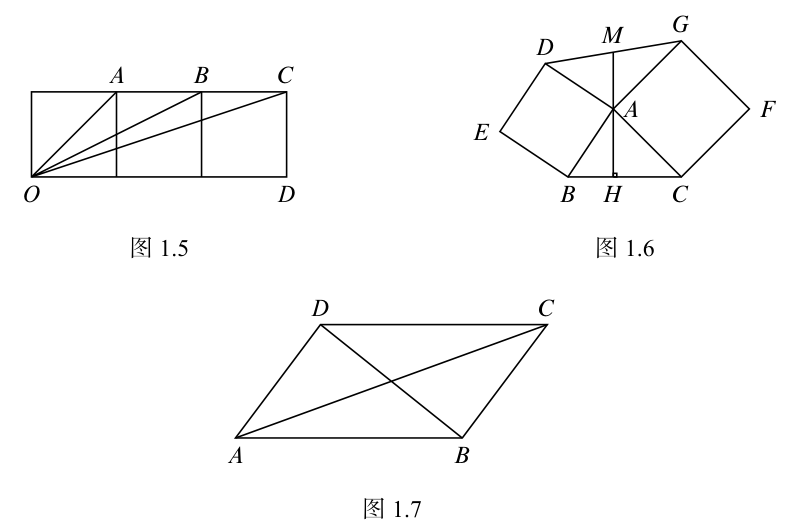
\includegraphics{public/figures/complex-functions/ch01-exercise-figures.png}
\caption{教材图 1.5、1.6、1.7，分别对应习题 1.2 第 7、8、9 题}
\end{figure}

\par\Needspace{5\baselineskip}
\noindent\textbf{10.} 证明

\[
|z_1+z_2|^2+|z_1-z_2|^2=2(|z_1|^2+|z_2|^2),
\]

并说明等式的几何意义。

\par\Needspace{5\baselineskip}
\noindent\textbf{11.} 设 \(z_1,\ldots,z_n\) 是单位圆周（以原点为中心、半径为
\(1\) 的圆周）上的 \(n\) 个点，如果它们是正 \(n\) 边形的 \(n\)
个顶点，证明 \(z_1+\cdots+z_n=0\)。

\par\Needspace{5\baselineskip}
\noindent\textbf{12.} 设 \(z_1,z_2,z_3\)
是单位圆周上的三个点，证明：这三个点是一正三角形三个顶点的充要条件为
\(z_1+z_2+z_3=0\)。

\par\Needspace{5\baselineskip}
\noindent\textbf{13.} 设 \(z_1,z_2,z_3,z_4\)
是单位圆周上的四个点，证明：这四个点是一矩形顶点的充要条件为
\(z_1+z_2+z_3+z_4=0\)。

校勘：第 12、13 题中作为顶点的点按互异理解，第 11
题按非退化正多边形理解。

\par\Needspace{5\baselineskip}
\noindent\textbf{14.} 设 \(L\) 是由方程

\[
az\bar z+\bar\beta z+\beta\bar z+d=0
\]

所确定的点的轨迹，其中 \(a,d\) 是实数，\(\beta\) 是复数。证明：

（1）当 \(a=0,\beta\ne0\) 时，\(L\) 是直线；

（2）当 \(a\ne0,|\beta|^2-ad>0\) 时，\(L\)
是一圆周，并求出其圆心和半径。

\par\Needspace{5\baselineskip}
\noindent\textbf{15.} 设 \(z_1\ne z_2\)、\(0<\lambda\ne1\)，证明由方程

\[
\left|\frac{z-z_1}{z-z_2}\right|=\lambda
\]

所确定的点 \(z\) 的轨迹是一圆周（通常称为 Apollonius 圆），该圆周的圆心
\(a\) 和半径 \(R\) 分别为

\[
a=\frac{z_1-\lambda^2z_2}{1-\lambda^2},\qquad
R=\frac{\lambda|z_1-z_2|}{|1-\lambda^2|}.
\]

并问 \(\lambda=1\) 时其轨迹是什么？

\par\Needspace{5\baselineskip}
\noindent\textbf{16.} 如果 \(z_1,\ldots,z_n\) 都位于过原点的直线的一侧，证明
\(1/z_1,\ldots,1/z_n\) 也必位于该直线的某一侧，且满足

\[
z_1+\cdots+z_n\ne0,\qquad
\frac1{z_1}+\cdots+\frac1{z_n}\ne0.
\]

校勘：原题``该直线''一般不正确，应改为``原直线关于实轴对称所得直线''；``一侧''指严格的同一侧。此处保留原句并提示修正，避免对错误命题作证明。

\par\Needspace{5\baselineskip}
\noindent\textbf{17.} 设 \(z_1,\ldots,z_n\) 是一个凸 \(n\) 边形的 \(n\)
个顶点，如果 \(a\) 满足

\[
\frac1{z_1-a}+\cdots+\frac1{z_n-a}=0,
\]

那么 \(a\) 必在这个凸 \(n\) 边形的内部。

\par\Needspace{5\baselineskip}
\noindent\textbf{18.} 证明：

\[
\sin\frac\pi n\sin\frac{2\pi}n\cdots\sin\frac{(n-1)\pi}n
=\frac n{2^{n-1}}.
\]

提示：考虑方程式 \((z+1)^n=1\) 的 \(n-1\) 个不为零的根的乘积。

\par\Needspace{5\baselineskip}
\noindent\textbf{19.} 设 \(0<\theta<\pi/2\)，

\[
P_m(x)=\sum_{k=0}^m(-1)^k\binom{2m+1}{2k+1}x^{m-k}.
\]

证明：\(\sin(2m+1)\theta=\sin^{2m+1}\theta\,P_m(\cot^2\theta)\)。

\par\Needspace{5\baselineskip}
\noindent\textbf{20.} 利用上题结果证明：

\[
\begin{aligned}
\text{(1)}\quad &\sum_{k=1}^m\cot^2\frac{k\pi}{2m+1}=\frac{m(2m-1)}3;\\
\text{(2)}\quad &\prod_{k=1}^m\cot^2\frac{k\pi}{2m+1}=\frac1{2m+1}.
\end{aligned}
\]

\Needspace{5\baselineskip}
\subsection{习题 1.3}\label{ux4e60ux9898-1.3}

教材第 13 页，共 6 题。

\par\Needspace{5\baselineskip}
\noindent\textbf{1.} 证明：在复数的球面表示下，\(z\) 和 \(1/\bar z\)
的球面像关于复平面对称。

\par\Needspace{5\baselineskip}
\noindent\textbf{2.} 证明：在复数的球面表示下，\(z\) 和 \(w\)
的球面像是直径对点当且仅当 \(z\bar w=-1\)。

校勘：乘积表达式用于有限非零复数；\(0\) 与 \(\infty\) 另成一对直径对点。

\par\Needspace{5\baselineskip}
\noindent\textbf{3.} 证明：在复数的球面表示下，\(\mathbb C_\infty\) 中的点
\(z,w\) 的球面像间的距离为

\[
\frac{2|z-w|}{\sqrt{(|z|^2+1)(|w|^2+1)}}.
\]

校勘：含 \(\infty\) 时按极限理解，不能直接代入未定义的
\(\infty/\infty\)。

\par\Needspace{5\baselineskip}
\noindent\textbf{4.} 证明：在复数的球面表示下，若
\(\begin{pmatrix}a&b\\c&d\end{pmatrix}\) 是二阶酉方阵，则
\(\mathbb C_\infty\) 的变换 \(w=(az+b)/(cz+d)\)
诱导了球面绕球心的一个旋转。

\par\Needspace{5\baselineskip}
\noindent\textbf{5.}
证明：在复数的球面表示下，球面上的圆周对应于复平面上的圆周或直线，反之亦然。

\par\Needspace{5\baselineskip}
\noindent\textbf{6.}
证明：在复数的球面表示下，复平面上两条光滑曲线在交点处的夹角与它们的球面像在交点处的夹角相等。

\Needspace{5\baselineskip}
\subsection{习题 1.4}\label{ux4e60ux9898-1.4}

教材第 14---15 页，共 5 题。

\par\Needspace{5\baselineskip}
\noindent\textbf{1.} 设
\(z_0\notin(-\infty,0]\)，\(z_n\ne0\)（\(\forall n\in\mathbb N\)）。证明：复数列
\(\{z_n\}\) 收敛到 \(z_0\) 的充要条件是 \(\lim_{n\to\infty}|z_n|=|z_0|\)
和 \(\lim_{n\to\infty}\arg z_n=\arg z_0\)。

\par\Needspace{5\baselineskip}
\noindent\textbf{2.} 设 \(z=x+iy\in\mathbb C\)，证明：

\[
\lim_{n\to\infty}\left(1+\frac zn\right)^n
=\mathrm e^x(\cos y+i\sin y).
\]

\par\Needspace{5\baselineskip}
\noindent\textbf{3.} 证明：如果 \(\lim_{n\to\infty}z_n=z_0\)，则

\[
\lim_{n\to\infty}\frac{z_1+z_2+\cdots+z_n}{n}=z_0.
\]

\par\Needspace{5\baselineskip}
\noindent\textbf{4.} 证明：若
\(\lim_{n\to\infty}z_n=z_0\)、\(\lim_{n\to\infty}w_n=w_0\)，则

\[
\lim_{n\to\infty}\frac1n\sum_{k=1}^n z_kw_{n-k}=z_0w_0.
\]

\par\Needspace{5\baselineskip}
\noindent\textbf{5.} 设无穷三角阵

\[
\begin{matrix}
a_{11}&&&\\
a_{21}&a_{22}&&\\
a_{31}&a_{32}&a_{33}&\\
\vdots&\vdots&\vdots&\ddots
\end{matrix}
\]

满足：

（1）对任意固定的 \(k\)，\(\lim_{n\to\infty}a_{nk}=a_k\) 存在；

（2）\(\lim_{n\to\infty}\sum_{k=1}^na_{nk}\) 存在；

（3）\(\sum_{k=1}^n|a_{nk}|\le M<\infty\)，\(\forall n\in\mathbb N\)。

证明：若复数列 \(\{z_n\}\) 收敛，则
\(\lim_{n\to\infty}\sum_{k=1}^na_{nk}z_k\) 存在。

\Needspace{5\baselineskip}
\subsection{习题 1.5}\label{ux4e60ux9898-1.5}

教材第 20 页，共 10 题。

\par\Needspace{5\baselineskip}
\noindent\textbf{1.} 证明：一个平面点集的孤立点的全体至多可列。

\par\Needspace{5\baselineskip}
\noindent\textbf{2.} 设 \(E\subset\mathbb C\)
是非空点集，\(z,w\in\mathbb C\)。证明 \(|d(z,E)-d(w,E)|\le|z-w|\)
成立，而 \(|d(z,E)-d(w,E)|\le d(z-w,E)\) 不成立。

\par\Needspace{5\baselineskip}
\noindent\textbf{3.} 指出下列点集的内部、边界、闭包和导集：

（1）\(\mathbb N=\{k:k\text{ 为自然数}\}\)；

（2）\(E=\{1/k:k\text{ 为自然数}\}\)；

（3）\(D=B(1;1)\cup B(-1;1)\)；

（4）\(G=\{z\in\mathbb C:1<|z|\le2\}\)；

（5）\(\mathbb C\)。

\par\Needspace{5\baselineskip}
\noindent\textbf{4.} 指出下列点集中哪些是开集，哪些是闭集，哪些是紧集：

（1）\(\mathbb Z=\{k:k\text{ 为整数}\}\)；

（2）\(E\) 为有限集；

（3）\(D=\{z\in\mathbb C:\operatorname{Im}z>0\}\setminus\bigl(\bigcup_{k=-\infty}^{\infty}F_k\bigr)\)，其中
\(F_k=\{z\in\mathbb C:z=k+iy,\ 0\le y\le1\}\)；

（4）\(G=B(0;1)\setminus\{1/(k+1):k\text{ 为自然数}\}\)；

（5）\(\mathbb C\setminus B(\infty;R)\)。

\par\Needspace{5\baselineskip}
\noindent\textbf{5.} 证明：若 \(D\) 为开集，则 \(D'=\bar D=\partial D\cup D\)。

\par\Needspace{5\baselineskip}
\noindent\textbf{6.} 设 \(\Lambda\) 是指标集，\(\{D_\alpha\}_{\alpha\in\Lambda}\)
是开集族，\(\{F_\alpha\}_{\alpha\in\Lambda}\)
是闭集族。证明：\(\bigcup_{\alpha\in\Lambda}D_\alpha\)
是开集，\(\bigcap_{\alpha\in\Lambda}F_\alpha\) 是闭集。

\par\Needspace{5\baselineskip}
\noindent\textbf{7.} 证明：有限个开集的交是开集，有限个闭集的并是闭集。

\par\Needspace{5\baselineskip}
\noindent\textbf{8.} 设 \(D\) 是开集，\(F\subset D\) 是非空紧集。证明：

（1）\(d(F,\partial D)>0\)；

（2）对任意 \(0<\delta<d(F,\partial D)\)，存在 \(F\) 中的点
\(z_1,\ldots,z_n\)，使得

\[
F\subset\bigcup_{k=1}^nB(z_k;\delta)\subset D,
\]

并且

\[
d\left(\bigcup_{k=1}^nB(z_k;\delta),\partial D\right)
\ge d(F,\partial D)-\delta.
\]

校勘：\(D=\mathbb C\) 时边界为空，需约定到空集距离为 \(+\infty\)，或另限
\(D\ne\mathbb C\)。

\par\Needspace{5\baselineskip}
\noindent\textbf{9.} 证明：若 \(E\) 是闭集，\(F\) 是紧集，则存在
\(z_0\in E,w_0\in F\)，使得 \(d(E,F)=|z_0-w_0|\)。将 \(F\)
换成闭集后是否还存在这样的 \(z_0,w_0\)？

校勘：本题须补充 \(E,F\) 非空。

\par\Needspace{5\baselineskip}
\noindent\textbf{10.} 证明：若 \(E\subset\mathbb C\) 既是开集，又是闭集，则 \(E\)
是空集或 \(E=\mathbb C\)。

\Needspace{5\baselineskip}
\subsection{习题 1.6}\label{ux4e60ux9898-1.6}

教材第 23---24 页，共 5 题。

\par\Needspace{5\baselineskip}
\noindent\textbf{1.} 满足下列条件的点 \(z\)
所组成的点集是什么？如果是域，说明它是单连通域还是多连通域？

（1）\(\operatorname{Re}z=1\)；

（2）\(\operatorname{Im}z<-5\)；

（3）\(|z-i|+|z+i|=5\)；

（4）\(|z-i|\le|2+i|\)；

（5）\(\arg(z-1)=\pi/6\)；

（6）\(|z|<1\)，\(\operatorname{Im}z>1/2\)；

（7）\(|(z-1)/(z+1)|\le2\)；

（8）\(0<\arg((z-i)/(z+i))<\pi/4\)。

\par\Needspace{5\baselineskip}
\noindent\textbf{2.} 证明：非空点集 \(E\subset\mathbb R\) 为连通集，当且仅当
\(E\) 是一个区间。

\par\Needspace{5\baselineskip}
\noindent\textbf{3.} 设 \(E\) 是非空点集，\(A\) 是 \(E\) 的非空子集。若 \(A\)
是连通的，并且不存在 \(E\) 的连通子集真包含 \(A\)，则称 \(A\) 是 \(E\)
的连通分支。证明：开集的连通分支仍然是开集，闭集的连通分支仍然是闭集。

\par\Needspace{5\baselineskip}
\noindent\textbf{4.} 设 \(E\) 是非空点集，\(\varepsilon>0\)。若对于 \(E\)
中任意两点 \(a,b\)，存在 \(E\) 中有限个点
\(a=z_0,z_1,\ldots,z_n=b\)，使得
\(|z_k-z_{k-1}|<\varepsilon\)（\(1\le k\le n\)），则称 \(E\) 为
\(\varepsilon\)-连通的。证明：紧集连通的充要条件是，对任意
\(\varepsilon>0\)，它都是
\(\varepsilon\)-连通的。并举例说明将紧集改为闭集后结论不再成立。

\par\Needspace{5\baselineskip}
\noindent\textbf{5.} 证明：若 \(D\) 是有界单连通域，则 \(\partial D\)
连通。举例说明，若 \(D\) 是无界单连通域，则 \(\partial D\) 可能不连通。

\Needspace{5\baselineskip}
\subsection{习题 1.7}\label{ux4e60ux9898-1.7}

教材第 26 页，共 9 题。

\par\Needspace{5\baselineskip}
\noindent\textbf{1.} 证明：若 \(E\) 是紧集，\(f:E\to\mathbb C\) 连续，则 \(f\) 在
\(E\) 上一致连续。

\par\Needspace{5\baselineskip}
\noindent\textbf{2.} 证明：若 \(D\) 是单连通域，\(0\notin D\)，则必存在 \(D\)
上的连续函数 \(\varphi(z)\)，使得
\(\varphi(z)\in\operatorname{Arg}z\)，\(\forall z\in D\)。\(\varphi(z)\)
称为 \(\operatorname{Arg}z\) 在 \(D\) 上的一个单值连续分支。

\par\Needspace{5\baselineskip}
\noindent\textbf{3.} 证明：若 \(E\) 是紧集，\(f\) 在 \(E\) 上连续，则 \(f(E)\)
也是紧集。将紧集换成闭集，结论是否成立？

\par\Needspace{5\baselineskip}
\noindent\textbf{4.} 设 \(f\) 是域 \(D\) 上的连续函数，并且对任意
\(z_0\in\partial D\)，\(\lim_{z\to z_0}f(z)\) 存在，证明

\[
F(z)=\begin{cases}
f(z),&z\in D,\\
\displaystyle\lim_{\zeta\to z}f(\zeta),&z\in\partial D
\end{cases}
\]

在 \(\bar D\) 上连续。

\par\Needspace{5\baselineskip}
\noindent\textbf{5.} 证明：若 \(f\) 在域 \(D\) 上一致连续，则对任意
\(z_0\in\partial D\)，\(\lim_{z\to z_0}f(z)\) 存在。

\par\Needspace{5\baselineskip}
\noindent\textbf{6.} 研究 \(f(z)=1/(1-z)\) 和 \(g(z)=1/(1+z^2)\) 在 \(B(0;1)\)
上的连续性与一致连续性。

\par\Needspace{5\baselineskip}
\noindent\textbf{7.} 设连续映射 \(f:E\to\mathbb C\) 满足
\(f(z)\ne f(w)\)（\(\forall z,w\in E,z\ne w\)），则称 \(f\) 是 \(E\)
上的一一连续映射。证明：若 \(E\) 是紧集，\(f\) 是 \(E\)
上的一一连续映射，则 \(f^{-1}:f(E)\to E\) 也是一一连续映射，即
\(f:E\to f(E)\) 是一个同胚映射。将紧集换成闭集，结论是否成立？

\par\Needspace{5\baselineskip}
\noindent\textbf{8.} 证明：

（1）存在连续映射将 \([0,1]\) 映为 \(\partial B(0;1)\)；

（2）不存在一一连续映射将 \([0,1]\) 映为 \(\partial B(0;1)\)。

\par\Needspace{5\baselineskip}
\noindent\textbf{9.} 设 \(f\) 是域 \(D\) 上的复变函数，\(z_0\in\partial D\)。若
\(\lim_{z\to z_0}f(z)=A\) 存在，则称 \(A\) 是 \(f\) 在 \(z_0\)
处的边界值，记为 \(f(z_0)=A\)。举例说明，存在开正方形 \(G\)
上的同胚映射，其不能在 \(\bar G\) 上处处都有边界值。

\end{document}
